\documentclass[16pt, letterpaper, titlepage]{article}
\usepackage[left=3.5cm, right=2.5cm, top=2.5cm, bottom=2.5cm]{geometry}
\usepackage[MeX]{polski}
\usepackage[utf8]{inputenc}
\usepackage{graphicx}
\usepackage{enumerate}
\usepackage{amsmath} %pakiet matematyczny
\usepackage{amssymb} %pakiet dodatkowych symboli
\title{Pierwszy dokument LaTeX}
\author{Małgorzata Klonowska}
\date{Październik 2022}
\begin{document}
\maketitle
\begin{huge}
\begin{center}
\textbf{pierwsze starcie w walce z pdfem}
\end{center}
\end{huge}
\newpage
\begin{LARGE}
\begin{enumerate}
\item teraz 
\item sobie
\item wypunktowuje
\item rzeczy
\end{enumerate}
\end{LARGE}
\newpage
\begin{quotation}
\section{brak umiejętności}
\subsection{przejawia się bezmózgiem totalnym}
\subsubsection{i niemożmożnością korzystania z prostych programów}
\end{quotation}
\newpage
\begin{center}
\begin{Huge}
\section*{przepis na szarlotkę amerykańską}
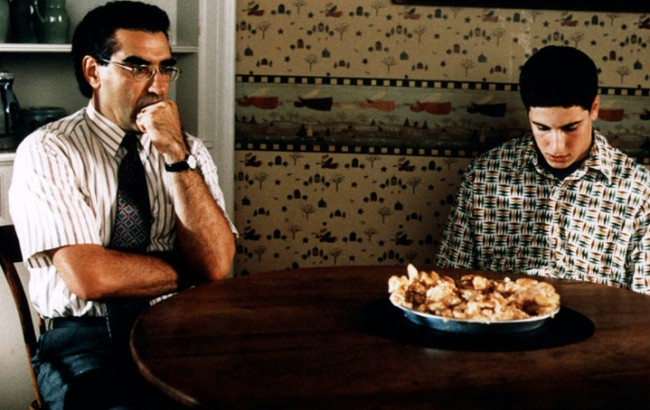
\includegraphics[scale=0.5]{szarlotka.jpg}
\end{Huge}
\begin{LARGE}
\subsection*{składniki}
\end{LARGE}
\subsubsection*{spód}
\end{center}
\begin{itemize}
\item 500 g mąki uniwersalnej
\item 250 g masła
\item 3/4 płaskiej łyżeczki soli
\item 50 g cukru pudru
\item 2 żółtka
\item ok. 100 ml wody
\item skórka z połowy cytryny
\end{itemize}
\begin{center}
\subsubsection*{nadzienie}
\end{center}
\begin{itemize}
\item 7-8 jabłek*
\item 60 g brązowego cukru
\item 30 g mąki uniwersalnej
\item 1 czubata łyżeczka cynamonu
\item spora szczypta gałki muszkatołowej
\item skórka z połowy cytryny
\item 1 rozbełtane jajko
\end{itemize}
\textbf{* Użyłam złotej renety, ale dobre są też szare renety, antonówki, czy inne “szarlotkowe” odmiany.}
\begin{center}
\begin{Large}
\subsection*{wykonanie}
\end{Large}
\end{center}
\begin{enumerate}
\item Zaczynamy od przygotowania kruchego spodu.
W tym celu do miksera wsypujemy mąkę, cukier puder, sól oraz pokrojone w kawałki miękkie masło. Mieszamy składniki do uzyskania mokrego piasku.
\item Dodajemy żółtka, wodę oraz skórkę z cytryny i ponownie zagniatamy aż pojawią się duże okruszki.
Naturalnie ciasto można zrobić również ręcznie, ale w mikserze jest dużo szybciej i masło nie nagrzewa się dodatkowo od rąk.
\item Wykładamy ciasto, a w zasadzie “okruchy” na folię spożywczą. Zwijamy w ciasną kulkę i wkładamy na min. 30-40 minut do lodówki.
\item W między czasie przygotowujemy nadzienie. Obieramy jabłka i pozbywamy się gniazd nasiennych. Kroimy na pół, a potem jeszcze w cienkie paski.
\item Przekładamy do dużej miski. Wsypujemy mąkę, cynamon, gałkę muszkatołową, cukier i skókę z cytryny. Mieszamy.
\item Wyciągamy ciasto z lodówki. Dzielimy na dwie części i wałkujemy. Staramy się przy tym, by ciasto miało kształt zbliżony do koła o średnicy min. 30 cm.
\item Jeśli ciasto się nieco klei możemy podsypać je mąką. Ułatwieniem jest silikonowa stolnica dzięki której cienko rozwałkowane ciasto łatwo daje się umieścić w wysmarowanej masłem formie. Ciasto dociskamy do formy i obcinamy jego nadmiar na brzegach.
\item Wykładamy pokrojone jabłka.

\textit{Moja uwaga:
Jabłka wykładamy “z czubem”, gdyż skurczą się w wysokiej temperaturze, a nie chcemy przecież, by ciasto było wklęsłe po upieczeniu.}
\item Drugą część ciasta również rozwałkowujemy i wycinamy długie paski o szerokości ok. 3 cm. Przeplatamy je ze sobą tworząc wzór kratki. Paski dociskamy na krawędziach do formy.
\item Z wierzchu szarlotkę smarujemy rozmąconym jajkiem. Dla ładniejszego efektu możemy jeszcze przyozdobić brzegi ciasta tworząc wzór np. za pomocą tępej strony noża.
\item Szarlotkę wstawiamy do piekarnika nagrzanego do 160 stopni C (z termoobiegiem) lub 180 stopni C (bez tej funkcji). Pieczemy ok. 55-60 minut aż ciasto się zezłoci.
\end{enumerate}
\begin{center}
\subsection*{podanie}
\end{center}
\textbf{Po wyjęciu z pieca szarlotka powinna stygnąć co najmniej 30 minut, a najlepiej całą godzinę. Jeśli pokroicie ją zbyt szybko będzie się rozlatywać, ale naturalnie będzie smakowała wybornie. Osobiście jednak zalecam uzbrojenie się w cierpliwość, bo wtedy efektem będą ładne i estetyczne kawałki.
Amerykańską szarlotkę często podaje się w towarzystwie lodów waniliowych lub waniliowego sosu.
Dla mnie jest jednak znakomita również bez żadnych dodatków.}
\end{document}